\section{LDU Design}

%$$$$$$$$$$$$$$$$$$$$$$$$$$$$$$$$$$$$$$$$$$$$$$$$$$$$$$$$$$$$$$$$$$$$$$$$$$$$$$$$
%Paragraph 1: LDU의 특징을 간단한 설명과 이번장에 대한 설명(LDU의 특징을 요약하여 설명)
%$$$$$$$$$$$$$$$$$$$$$$$$$$$$$$$$$$$$$$$$$$$$$$$$$$$$$$$$$$$$$$$$$$$$$$$$$$$$$$$$

%LDU는 리눅스 커널의 high update rates를 가진 data strcuture의 Scalability 위한 
%새로운 로그 기반의  위한 Concurrent Updates 방법이다. LDU는 timestamp를
% 이용하여 발생하는 log를 관리에 대한 어려움을 해결하였다. 
%
%time-stamp를 사용하지 않기 위해 LDU는 최소한의 shared memory system 
%atomic 연산을 사용하도록 하여 설계하였다. 
%이러한 LDU의 기본적인 철학은 distributed system에서 주로 사용하는 time-stamp log기반 
%방식의 concurrent updates 방법과 shared memory system에서만 사용할 수 있는 CAS와 같은
%atomic operation을 절묘하게 결합하여 설계하였다. 
% 즉 저장된 log를 consistency를 유지하기 위해 최소한의 atomic operation을 사용하도록 설계하였다. 
%LDU는 cache invalidate 줄이기(mitigating)을 최소화 하기 위해 
%3가지 방법(light weight queue,  Update-side Abosrbing, reusing garbage object)을 
%병행 하였다.

LDU 
This section explains these algorithmic design aspects of LDU.

\subsection{Log-based Concurrent updates}

%$$$$$$$$$$$$$$$$$$$$$$$$$$$$$$$$$$$$$$$$$$$$$$$$$$$$$$$$$$$$$$$$$$$$$$$$$$$$$$$$
%Paragraph 1: Log 기반의 알고리즘 설명 
%$$$$$$$$$$$$$$$$$$$$$$$$$$$$$$$$$$$$$$$$$$$$$$$$$$$$$$$$$$$$$$$$$$$$$$$$$$$$$$$$

%Update heavy한 구조 때문에 발생하는 scalability 문제에 대한 해결 책 중 하나는
%Log기반의 알고리즘을 사용하는 것이다. Log-based 알고리즘은 lock을 피하기 위해
%update가 발생하면, data structure의 update operation(insert or remove)을 argument와 함께
% 저장하고, 주기적 또는 before a read operation에 applies the updates in all the
%logs to the data structure, so reader can read up to date data structure.
%Log-based 방법은 마치 CoW(Copy on Write)와 같이, read 전에 저장된 log가 수행됨으로
% read가 간혈적으로 수행되는 data structure에 적합한 방법이다.


%$$$$$$$$$$$$$$$$$$$$$$$$$$$$$$$$$$$$$$$$$$$$$$$$$$$$$$$$$$$$$$$$$$$$$$$$$$$$$$$$
%Paragraph 2: Log 기반의 알고리즘의 장점
%$$$$$$$$$$$$$$$$$$$$$$$$$$$$$$$$$$$$$$$$$$$$$$$$$$$$$$$$$$$$$$$$$$$$$$$$$$$$$$$$
%
%Log-based 방법은 총 4가지의 장점을 가진다. 첫째로, Update가 수행하는 시점
%로그를 저장하는 순간에는 Lock이 필요가 없다. 
%둘째로, 저장된 Log를 corse-grain Lock과 함께 하나의 코어에서 수행하므로 
%cache에 효율성이 높아진다. 또한 OpLog와 같이 log를 per-core로 저장하면, cache
%invalidate에 대한 오버헤드를 최소화 할 수 있다. 
%셋째로, 기존 여러 데이터 structure에 쉽게 적용할 수 있는 장점이 있다.
%마지막으로 저장된 Log를 실제 수행하지 않고, 여러가지 optimization 방법을 사용하여
%적은 operation으로 Log를 줄일 수 있다.

Log-based approaches can help to support high update rates because


\subsection{Approach}

%$$$$$$$$$$$$$$$$$$$$$$$$$$$$$$$$$$$$$$$$$$$$$$$$$$$$$$$$$$$$$$$$$$$$$$$$$$$$$$$$
%Paragraph 1: LDU는 another CoW 기법 : read before physical update 
%$$$$$$$$$$$$$$$$$$$$$$$$$$$$$$$$$$$$$$$$$$$$$$$$$$$$$$$$$$$$$$$$$$$$$$$$$$$$$$$$

%LDU도 log-based approach를 가진다 그러므로 log-based 방법의 장점을 모두 가진다.
%LDU는 먼저 lock 없이 Concurrent Updates를 위해 수행 시점에서는 Atomic하게 Operation
% Log를 Global queue에 저장 한다. Lock이 필요 없어 scalability가 뿐만 아니라 
% Lock 자체의 오버헤를 줄일 수 있다. 
%Log를 저장하는 저장된 Log는 주기적으로 또는 read 전에 호출되게 되는데, 
%LDU는 FC와 같이 operation Log를 corse grain lock과 함께 single core에서 수행하므로 
%cache의 miss를 줄여 성능을 향상시킨다.
%또한 LDU는 Log-based 방법과 같이 기존 data structure를 많이 수정하지 않아
%다른 data structure에 쉽게 적용할 수 있다.
%LDU가 global queue를 사용함에 따라, CAS operations on
% the head of the queue limit scalability(the bottleneck on the log is similar
% to that the Michael and Scott queue) 이처럼 LDU는 global queue의 사용에 대한 cache
% invalidate 줄이고, 불필요한 연산을 줄이기 위해, CAS를 최소화한 queue를 사용, update-side absorbing,
% reusing garbage object 등과 같이 3가지 optimization을 수행하였다. 


For update-heavy data structure LDU update before read operation;for example, it
similar to CoW(Copy On Write) method because acture update as long as possible
late.


%$$$$$$$$$$$$$$$$$$$$$$$$$$$$$$$$$$$$$$$$$$$$$$$$$$$$$$$$$$$$$$$$$$$$$$$$$$$$$$$$
%Paragraph 2: GLDU: Global queue 를 활용하는 Log 기반 방법 
%$$$$$$$$$$$$$$$$$$$$$$$$$$$$$$$$$$$$$$$$$$$$$$$$$$$$$$$$$$$$$$$$$$$$$$$$$$$$$$$$

% LDU는 global queue의 head 포인터에 대한 CAS 연산을 최대한 줄이기 위해 
% log를 저장하고자 하는 큐를 multiple producers and single consumer에 기반하는
% non-blocking queue를 이용하였다. 이 큐는 다른 non-blocking list와 다르게
% insert operation을 head의 first 노드에 삽입함에 따라, CAS가 발생되는 횟수가 
% 상대적으로 적다. 게다가 remove를 위한 복잡한 알고리즘이 필요없다. 그 이유는 저장된 log를 
% 수행하는 single consumer는 head  pointer를 NULL로 xchg 명령을 사용하여 atomic하게 제거한다.
% 따라서 remove를 위한 복잡한 알고리즘이 필요없다.
% 이러한 큐는 이미 Linux 커널에 Lock-less list라는 이름으로 구현되어 있으며, 
% 이미 커널에 많은 부분에 사용되고 있다. LDU도 Linux 커널에 있는 Lock-less list를 활용 하였다. 




%$$$$$$$$$$$$$$$$$$$$$$$$$$$$$$$$$$$$$$$$$$$$$$$$$$$$$$$$$$$$$$$$$$$$$$$$$$$$$$$$
%Paragraph 3: PLDU: Per-core lock-less list를 활용하는 Log 기반 방법
%$$$$$$$$$$$$$$$$$$$$$$$$$$$$$$$$$$$$$$$$$$$$$$$$$$$$$$$$$$$$$$$$$$$$$$$$$$$$$$$$

%







%$$$$$$$$$$$$$$$$$$$$$$$$$$$$$$$$$$$$$$$$$$$$$$$$$$$$$$$$$$$$$$$$$$$$$$$$$$$$$$$$
%Paragraph 4: PLDU의 Insert-Remove Operation에 대한 처리 설명 - time ordering
%$$$$$$$$$$$$$$$$$$$$$$$$$$$$$$$$$$$$$$$$$$$$$$$$$$$$$$$$$$$$$$$$$$$$$$$$$$$$$$$$

% * object에 대한 순서가 만약 Insert와 remove가 변경된다면, 문제가 발생한다. 
%If a process logs an insert operation on one core,
%migrates to another core, and logs a remove operation, the remove should
%eventually execute after the insert[OpLog].










%$$$$$$$$$$$$$$$$$$$$$$$$$$$$$$$$$$$$$$$$$$$$$$$$$$$$$$$$$$$$$$$$$$$$$$$$$$$$$$$$
%Paragraph 5: optimization point one : Update-side Abosrbing 
%$$$$$$$$$$$$$$$$$$$$$$$$$$$$$$$$$$$$$$$$$$$$$$$$$$$$$$$$$$$$$$$$$$$$$$$$$$$$$$$$
% 로그를 집어 넣을 때 체크를 하여 xchg atomic 연산을 활용하여 operation을 지우는 방법

% LDU는 최적화를 위해 update-side absorbing이라는 방법을 사용한다. Update operation는 
% 만약 같은 object에 대해서 insert와 remove가 발생하였으면, 같은 object에 대해서는
% insert oepration과 remove operation은 수행을 안해도 되는 operation이다. 
% 이러한 방법은 log 기반으로 deferred 로 수행하기 떄문에 가능한것인데, 
% log로 저장을 했기 때문에 삭제가 가능한 operation을 삭제하여 성능을 높이는 방법이다.
% OpLog는 이러한 Log 삭제를 같은 코어서 동작하면 적은 operation으로 바로 바로 삭제를 
% 하나 다른 코어로
% 이동된 Log 같은 경우 삭제를 위해 검색을 해야하는 추가적인 작업을 수행하는 문제가 있다.
% LDU는 Log를 줄이는 작업에는 shared memory system의 atomic operation을 사용하였다.
% LDU는 모든 object에 insert와 remove의 mark 필드를 추가해서 
% global head 포인터에 비싼 CAS연산을 사용을 줄이는 방법을 사용한다.
% 이것은 삭제가능한 operationg일 경우 CAS를 사용하여 로그로 저장하지 않고
% update를 수행할 때 SWAP operation을 활용해 바로 바로 지워주는 알고리즘을 사용하였다. 
% 예를 들어 만약
% A라는 object를 대상으로 insert-remove operation이 수행될 경우 처음 insert
% operation은 insert mark 필드에 표시하고 queue에 저장한다. 다음 remove
% operation 부터는 log를 queue에 저장하지 않고 insert에 표시한 mark 필드에 표시한
% 값만 지워주는 방식으로 사용한다. 이것은 상대적으로 가벼운 연산만 사용해서 
% log를 지워주는 효과를 가져주므로 성능 향상을 준다.





%$$$$$$$$$$$$$$$$$$$$$$$$$$$$$$$$$$$$$$$$$$$$$$$$$$$$$$$$$$$$$$$$$$$$$$$$$$$$$$$$
%Paragraph 6: optimization point two : reusing garbage object 
%$$$$$$$$$$$$$$$$$$$$$$$$$$$$$$$$$$$$$$$$$$$$$$$$$$$$$$$$$$$$$$$$$$$$$$$$$$$$$$$$

% LDU의 또 다른 최적화 기법은 update-side absorbing 때문에 취소된 
% garbage object를 재활용하는 것이다. 이것은 queue에는 존재하만 update-side
% aborsrbing 때문에 취소 되어 garbage가 되어 queue에 보관되어 있는 log일 경우, 
% 다음 update operation에
% 대해서는 로그를 새로 많들어 넣지 않고 기존 로그를 재활용하는 방법이다. 
% 예를 들어  같은 오브젝트에 대해서 insert-remove-insert 순서로 update가 수행될
% 경우에는 세번째 insert 명령어는 global operation list에 들어가 있지만 remove가 발생하여
% mark filed가 zero인 경우(garbage object)이다. 이러한 경우 다음 insert operation에 대해서
% 비싼 연산인 list에 연산을 다시 넣지 않고, 해당 object의 mark 필드만
% 변경하여 log를 재활용하는 방법을 사용하였다. 


%$$$$$$$$$$$$$$$$$$$$$$$$$$$$$$$$$$$$$$$$$$$$$$$$$$$$$$$$$$$$$$$$$$$$$$$$$$$$$$$$
%Paragraph 7: 중간에 한번씩 log를 flush
%$$$$$$$$$$$$$$$$$$$$$$$$$$$$$$$$$$$$$$$$$$$$$$$$$$$$$$$$$$$$$$$$$$$$$$$$$$$$$$$$

%To keep the log from growing without end, log-based method periodically 
% apply the time-ordered operations at the head of the log to remove these
% opearation from the log. LDU는 주기적으로 Log를 적용함으로 Log가 쌓여서
% 발생하는 메모리 낭비를 줄인다.






%$$$$$$$$$$$$$$$$$$$$$$$$$$$$$$$$$$$$$$$$$$$$$$$$$$$$$$$$$$$$$$$$$$$$$$$$$$$$$$$$
%Paragraph 8: LDU limitation 설명
%$$$$$$$$$$$$$$$$$$$$$$$$$$$$$$$$$$$$$$$$$$$$$$$$$$$$$$$$$$$$$$$$$$$$$$$$$$$$$$$$

% LDU는 2가지 limitation을 가지고 있다. 

% 첫번째로는 리눅스 커널과 같이 
% search가 two update operations(one to insert and one to remove an element) 함수
% 외부해서 수행하는 data structure에만 적용이 가능하다.
% 즉 다시말하면 리눅스의 data structure의 경우에는 search와 update가 분리되어 있어
% 같은 update operation이 연달아 호출되지 않는다.
% 즉 이러한 구조는 search가 외부에 있기 때문에 insert operation 다음에는 반드시 
% remove opration이 발생하고 
% remove operation 다음에는 반드시 insert operation이 발생하는 특징이 있다.

% 이와 반대로 research 분야에서 많이 연구되는 CSDS(Concurrent search data structures)[]의 
% 방법들은 search가 update operation 내부에 존재하는 구조로 되어 있어서
% 같은 노드에 대해서 insert-insert 또는 remove-remove 순서로 동작할 수 있다.
% 이러한 경우에는 LDU를 적용하지 못한다.

% 하지만 CSDS 구조가 아닌 data structure를 사용하여 


\subsection{LDU example}

\subsubsection{GLDU example}
%$$$$$$$$$$$$$$$$$$$$$$$$$$$$$$$$$$$$$$$$$$$$$$$$$$$$$$$$$$$$$$$$$$$$$$$$$$$$$$$$
%Paragraph 1: GLDU Flowchart 그림 설명 
%$$$$$$$$$$$$$$$$$$$$$$$$$$$$$$$$$$$$$$$$$$$$$$$$$$$$$$$$$$$$$$$$$$$$$$$$$$$$$$$$
%

\begin{figure}[tb]
  \begin{center}
     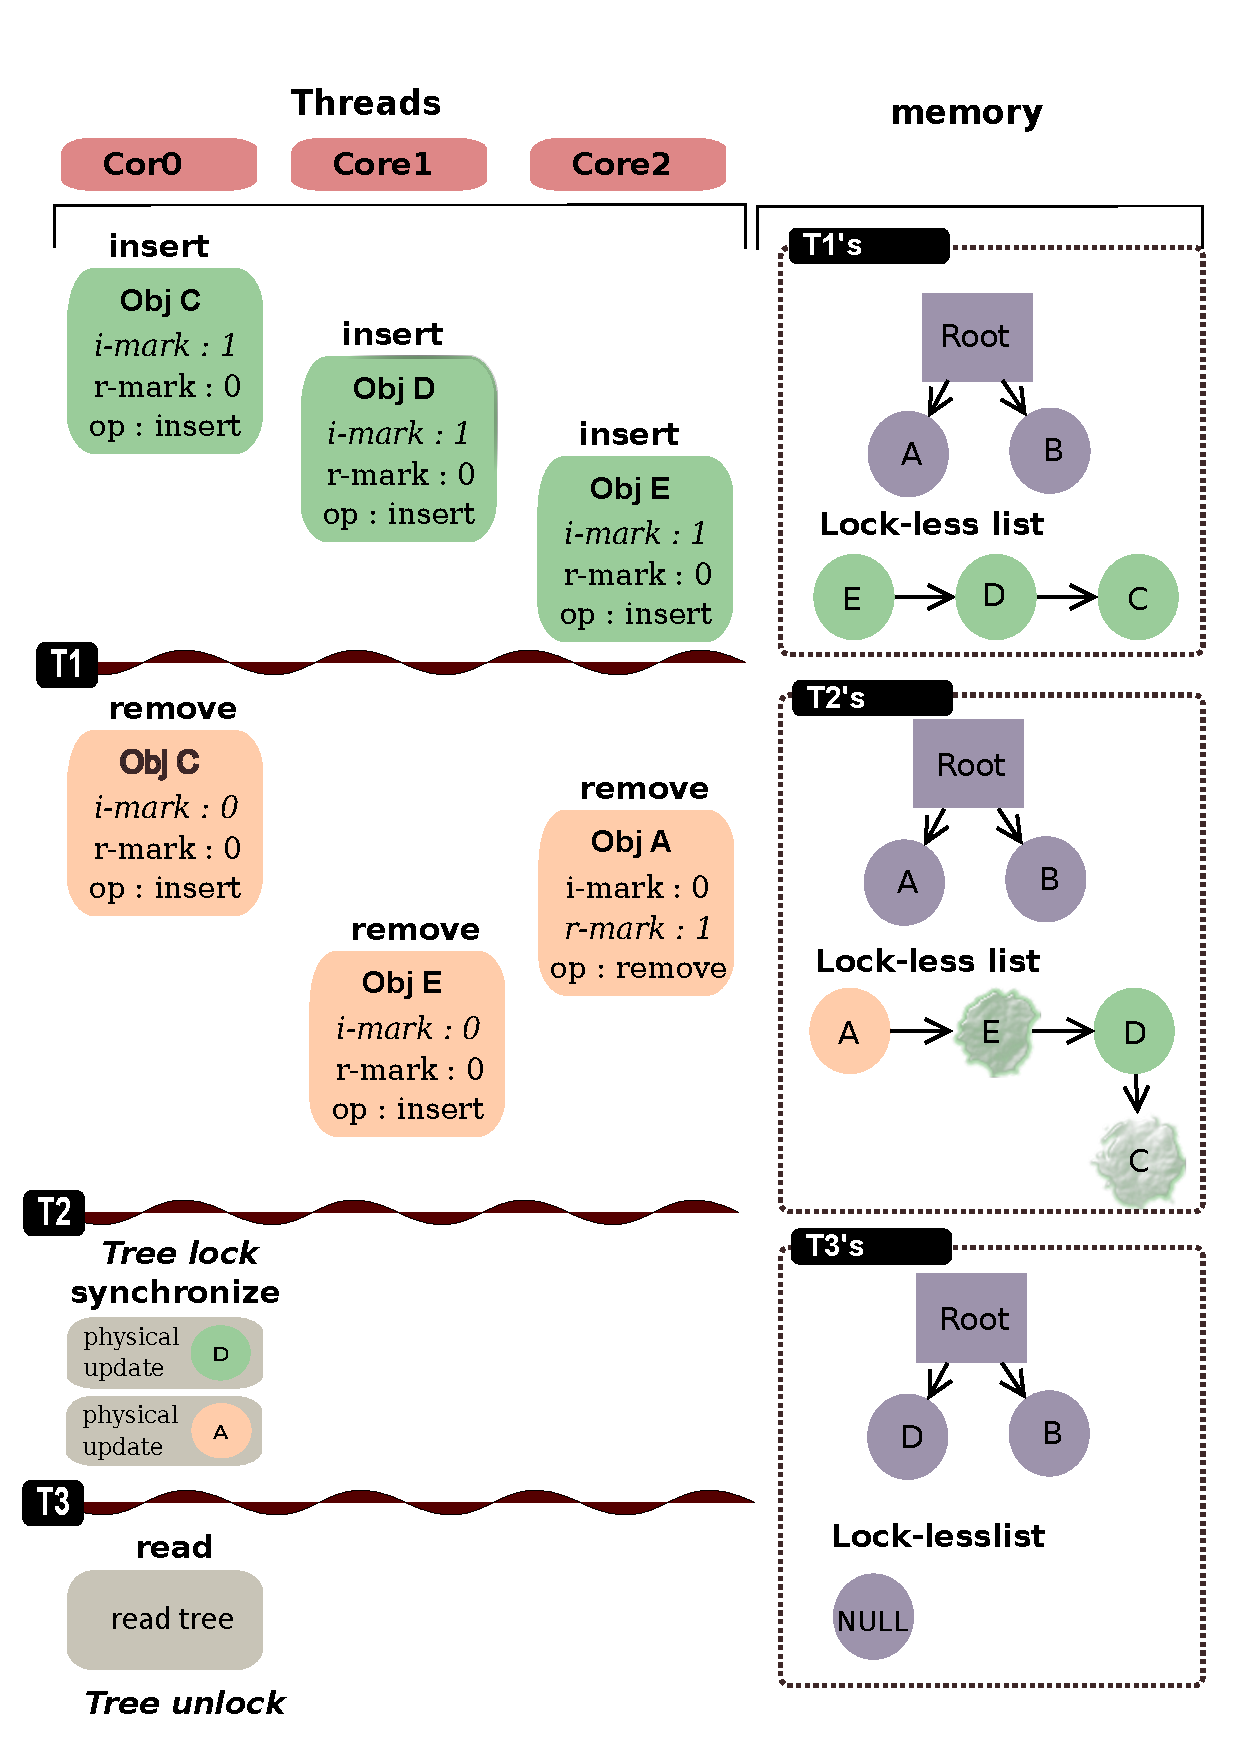
\includegraphics[width=0.5\textwidth,height=0.5\textheight,keepaspectratio]{fig/basic}
  \end{center}
  \caption{\deferu example showing six update operations and one read
  operation. The execution flows from top to bottom. Memory represents original
  data structure and logging queue at T1, T2 and T3, respectively.}
  \label{fig:basic}
\end{figure}


Figure \ref{fig:basic} gives an example of deferred update with six update
operations and one read operation.
In this figure, execution flows from top to bottom.
The data structure for \emph{physical update} is a tree, and initial values in
the tree are node \code{A} and \code{B}.
In contrast, the data structure for \emph{logical update} is lock-less list.
In the top figure, \code{Core0}, \code{Core1} and \code{Core2} perform the
logical insert operation to nodes \code{C}, \code{D} and \code{E},
 respectively.
The logical inserts set the insert mark, and they then insert their
nodes into lock-less list.
In this case, none of the lock is needed because \deferu uses the lock-less
list;all threads can execute the update concurrently.
At \code{T1}, the tree contains node \code{A}
and \code{B} and 
the lock-less list contains node \code{E}, \code{D} and \code{C}.
When removing the node \code{C}, the node \code{C}, whose mark field was marked
by insert, atomically cleans up the insert marked field.
At \code{T2}, the lock-less list contains nodes
\code{A}, \code{E}, \code{D}, and \code{C}, and the marking field is zero for 
nodes \code{E} and \code{C}.
Before running the \code{synchronize} function, they need to lock the original
 tree's lock using the exclusive lock in order to protect the tree's
 operation.
The \code{synchronize} migrates from lock-less list node to tree node, each of 
which is the marked node, so nodes \code{A} and \code{D} are migrated.
Finally, the tree contains nodes \code{D} and \code{B}, so the reader can read
 eventually consistent data.



\subsubsection{PLDU example}
%$$$$$$$$$$$$$$$$$$$$$$$$$$$$$$$$$$$$$$$$$$$$$$$$$$$$$$$$$$$$$$$$$$$$$$$$$$$$$$$$
%Paragraph 2: PLDU Flowchart 그림 설명 
%$$$$$$$$$$$$$$$$$$$$$$$$$$$$$$$$$$$$$$$$$$$$$$$$$$$$$$$$$$$$$$$$$$$$$$$$$$$$$$$$
%

\begin{figure}[tb]
  \begin{center}
     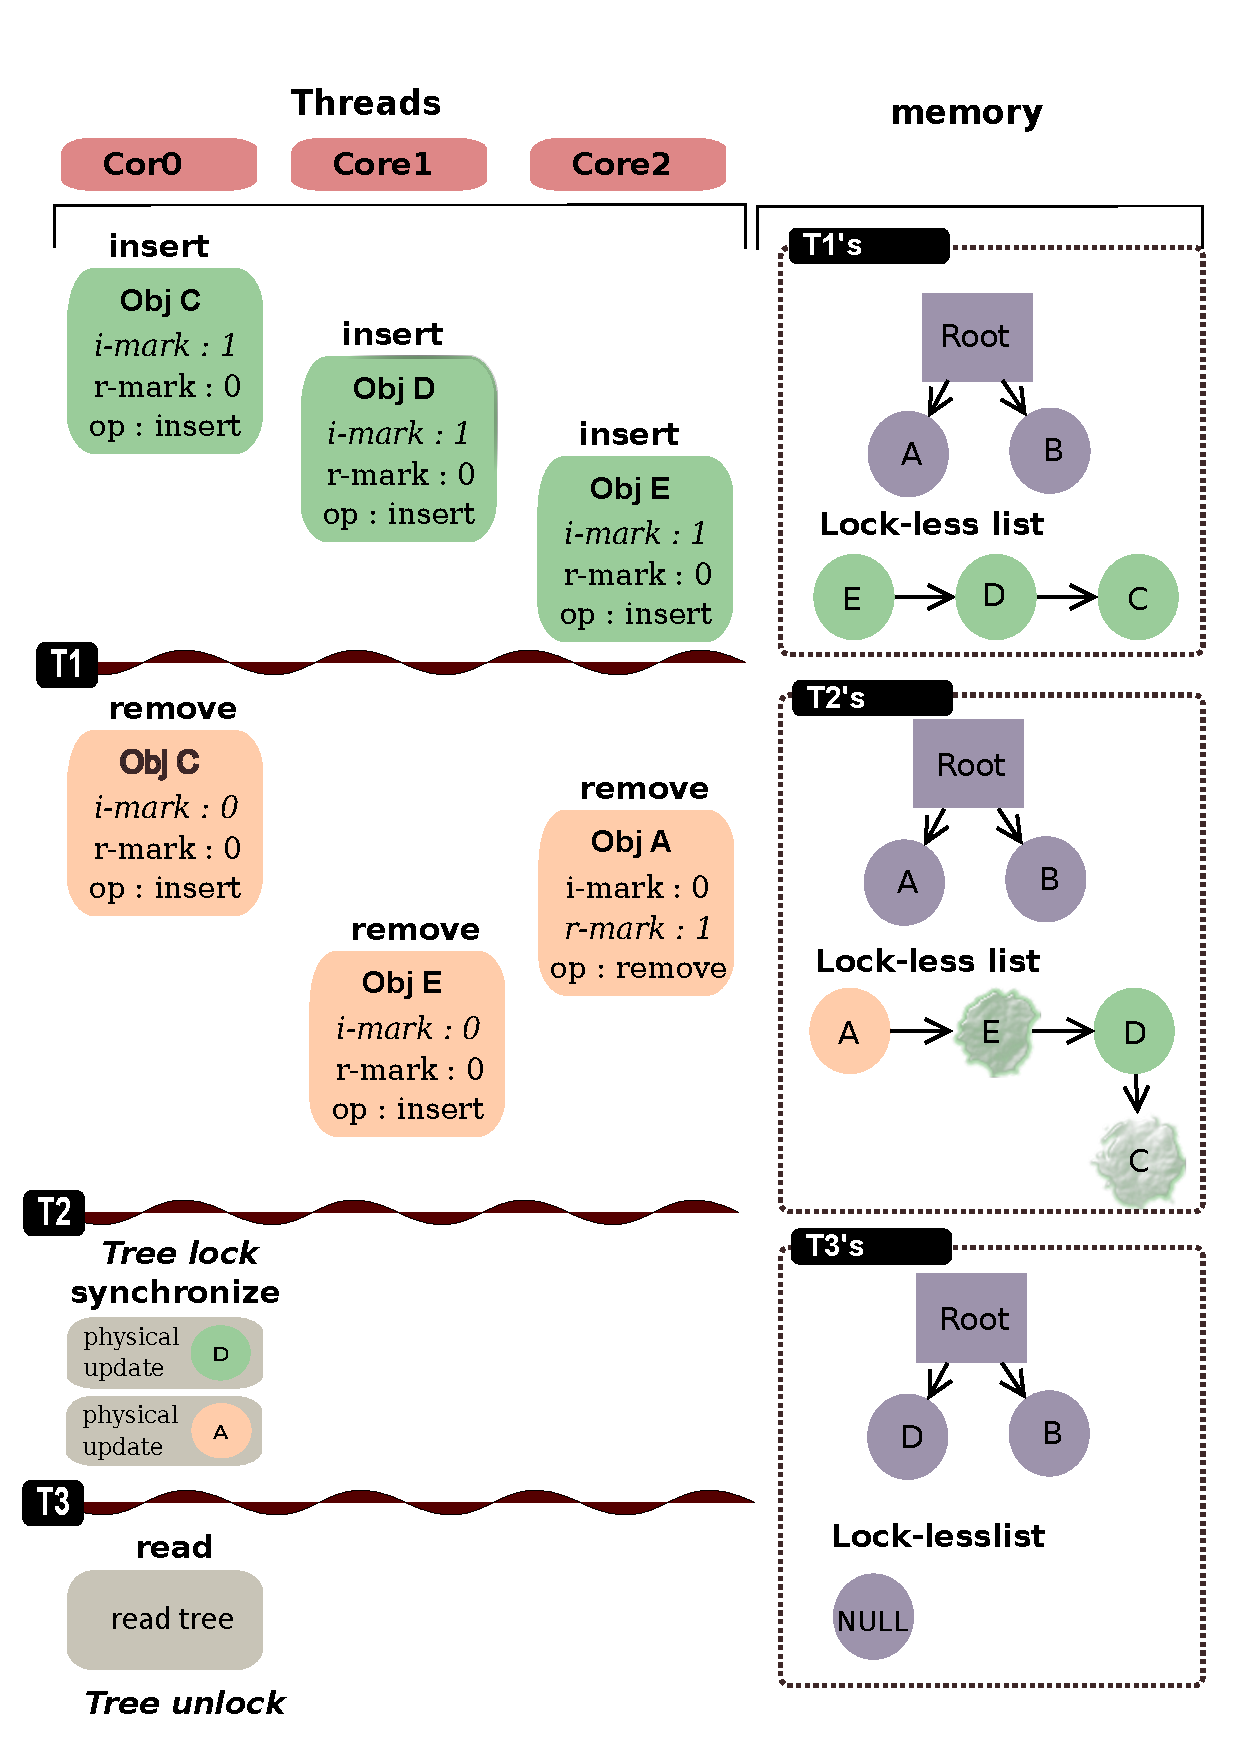
\includegraphics[width=0.5\textwidth,height=0.5\textheight,keepaspectratio]{fig/basic}
  \end{center}
  \caption{\deferu example showing six update operations and one read
  operation. The execution flows from top to bottom. Memory represents original
  data structure and logging queue at T1, T2 and T3, respectively.}
  \label{fig:basic}
\end{figure}


Figure \ref{fig:basic} gives an example of deferred update with six update
operations and one read operation.
In this figure, execution flows from top to bottom.
The data structure for \emph{physical update} is a tree, and initial values in
the tree are node \code{A} and \code{B}.
In contrast, the data structure for \emph{logical update} is lock-less list.
In the top figure, \code{Core0}, \code{Core1} and \code{Core2} perform the
logical insert operation to nodes \code{C}, \code{D} and \code{E},
 respectively.
The logical inserts set the insert mark, and they then insert their
nodes into lock-less list.
In this case, none of the lock is needed because \deferu uses the lock-less
list;all threads can execute the update concurrently.
At \code{T1}, the tree contains node \code{A}
and \code{B} and 
the lock-less list contains node \code{E}, \code{D} and \code{C}.
When removing the node \code{C}, the node \code{C}, whose mark field was marked
by insert, atomically cleans up the insert marked field.
At \code{T2}, the lock-less list contains nodes
\code{A}, \code{E}, \code{D}, and \code{C}, and the marking field is zero for 
nodes \code{E} and \code{C}.
Before running the \code{synchronize} function, they need to lock the original
 tree's lock using the exclusive lock in order to protect the tree's
 operation.
The \code{synchronize} migrates from lock-less list node to tree node, each of 
which is the marked node, so nodes \code{A} and \code{D} are migrated.
Finally, the tree contains nodes \code{D} and \code{B}, so the reader can read
 eventually consistent data.



\subsection{GLDU vs. PLDU}

%$$$$$$$$$$$$$$$$$$$$$$$$$$$$$$$$$$$$$$$$$$$$$$$$$$$$$$$$$$$$$$$$$$$$$$$$$$$$$$$$
%Paragraph 1: 둘간의 장단점 설명
%$$$$$$$$$$$$$$$$$$$$$$$$$$$$$$$$$$$$$$$$$$$$$$$$$$$$$$$$$$$$$$$$$$$$$$$$$$$$$$$$




\subsection{The LDU Algorithm}


\subsubsection{GLDU logical update}
%$$$$$$$$$$$$$$$$$$$$$$$$$$$$$$$$$$$$$$$$$$$$$$$$$$$$$$$$$$$$$$$$$$$$$$$$$$$$$$$$
%Paragraph 1:LDU Concurrent Updates 알고리즘 코드 및 설명 
%$$$$$$$$$$$$$$$$$$$$$$$$$$$$$$$$$$$$$$$$$$$$$$$$$$$$$$$$$$$$$$$$$$$$$$$$$$$$$$$$

The pseudo code for \deferu's \emph{logical update} is given in
figure~\ref{fig:logicalupdate}.
The \code{logical\_insert}, the concurrent update function, checks whether this
object already has been removed by \code{logical\_remove}.
If this object has been removed, \code{logical\_insert} initializes the marking
 field and then they return, which is fastpath.
The marking field needs synchronization because this field in the
\emph{logical update} is shared with the \emph{physical update}, so the CAS
 operation is needed.
When the marking field has been initialized, they set the
marking field, then they check whether or not this node already has been
 inserted in lock-less list.
If the node does not exist in lock-less list, then they insert the node into
lock-less list.

\begin{figure}[tb!]
\begin{obeylines}
\begin{obeyspaces}

\lstinputlisting{src/ldu_logical.c}
\end{obeyspaces}
\end{obeylines}
\rule{\columnwidth}{0.5pt}
\vspace{-\baselineskip}
\caption{\deferu logical update algorithm. \code{logical\_insert} represents
 non-blocking insert function.
It may be called by original insert position without locks. The fastpath is
 that when their object was removed by \code{logical\_remove},
 \code{logical\_insert} just changes node's marking field.}
\label{fig:logicalupdate}
\end{figure}


\subsubsection{GLDU Physical update}
%$$$$$$$$$$$$$$$$$$$$$$$$$$$$$$$$$$$$$$$$$$$$$$$$$$$$$$$$$$$$$$$$$$$$$$$$$$$$$$$$
%Paragraph 2:LDU Deferred Updates 알고리즘 코드 및 설명 
%$$$$$$$$$$$$$$$$$$$$$$$$$$$$$$$$$$$$$$$$$$$$$$$$$$$$$$$$$$$$$$$$$$$$$$$$$$$$$$$$

The pseudo code for \deferu's \emph{physical update} is given in
Figure~\ref{fig:physicalupdate}.
First, they check whether lock-less list is an empty list or not, then they
iterate the lock-less list.
If the marking field has been set, they execute migration from
lock-less to original data structure.
Because the marking field in \emph{physical update} is shared with
 \emph{logical update}, the CAS operation is needed.
They initialize the used field, which needs to protect the object from freed
 through destructor.
The programmer must acquire locks on the \code{synchronize\_ldu} function,
which migrates log to original data structure.
Finally, the \code{physical\_update} executes original functions by using the
operation log.

\begin{figure}[tb!]
\begin{obeylines}
\begin{obeyspaces}

\lstinputlisting{src/ldu_physical.c}

\end{obeyspaces}
\end{obeylines}
\rule{\columnwidth}{0.5pt}
\vspace{-\baselineskip}
\caption{\deferu physical update algorithm. \code{synchronize\_ldu} may be
 called by reader and converts update log to original data structure
 traversing the lock-less list.}
\label{fig:physicalupdate}
\end{figure}



\subsubsection{The PLDU Algorithm}

\begin{figure}[tb!]
\begin{obeylines}
\begin{obeyspaces}

\lstinputlisting{src/pldu_logical.c}
\end{obeyspaces}
\end{obeylines}
\rule{\columnwidth}{0.5pt}
\vspace{-\baselineskip}
\caption{\deferu logical update algorithm. \code{logical\_insert} represents
 non-blocking insert function.
It may be called by original insert position without locks. The fastpath is
 that when their object was removed by \code{logical\_remove},
 \code{logical\_insert} just changes node's marking field.}
\label{fig:logicalupdate}
\end{figure}


\subsubsection{PLDU logical update}


%$$$$$$$$$$$$$$$$$$$$$$$$$$$$$$$$$$$$$$$$$$$$$$$$$$$$$$$$$$$$$$$$$$$$$$$$$$$$$$$$
%Paragraph 1: object 기반 Hash table 관리 설명
%$$$$$$$$$$$$$$$$$$$$$$$$$$$$$$$$$$$$$$$$$$$$$$$$$$$$$$$$$$$$$$$$$$$$$$$$$$$$$$$$

% * 만약 LDU의 log를 저장하는 global object를 대상으로 per-core hash table로 object를 관리
%를 하면 장점이 있다.





\begin{figure}[tb!]
\begin{obeylines}
\begin{obeyspaces}

\lstinputlisting{src/pldu_physical.c}

\end{obeyspaces}
\end{obeylines}
\rule{\columnwidth}{0.5pt}
\vspace{-\baselineskip}
\caption{\deferu physical update algorithm. \code{synchronize\_ldu} may be
 called by reader and converts update log to original data structure
 traversing the lock-less list.}
\label{fig:physicalupdate}
\end{figure}





%$$$$$$$$$$$$$$$$$$$$$$$$$$$$$$$$$$$$$$$$$$$$$$$$$$$$$$$$$$$$$$$$$$$$$$$$$$$$$$$$
%Reference Sentence 1
%$$$$$$$$$$$$$$$$$$$$$$$$$$$$$$$$$$$$$$$$$$$$$$$$$$$$$$$$$$$$$$$$$$$$$$$$$$$$$$$$

* By default OpLog executes logged updates in temporal order. For example,
consider a linked list. If a process logs an insert operation on one core,
migrates to another core, and logs a remove operation, the remove should
eventually execute after the insert.
* OpLog relies on timestamps from a system-wide synchronized clock to tell it
how to order entries in different cores' log.
*This ordering ensures linearizaility, making OpLog compatible with existing
data structure semantics.



%$$$$$$$$$$$$$$$$$$$$$$$$$$$$$$$$$$$$$$$$$$$$$$$$$$$$$$$$$$$$$$$$$$$$$$$$$$$$$$$$
%Reference Sentence 1
%$$$$$$$$$$$$$$$$$$$$$$$$$$$$$$$$$$$$$$$$$$$$$$$$$$$$$$$$$$$$$$$$$$$$$$$$$$$$$$$$

%To keep the log from growing without end, we can at any point apply in-order a
%subsequence of the operations at the head of the log to the state to derive a
%new state, and remove these operation from the log[EuroSys 2006 PLS].

%High level operations performed on shared data structures can be divided into
%three groups: read-only, write-only, and read-modify-write[PLS].

%Read-only operations do not mutate the data, write-only operations modify the
%data but do not return a result, and read-modify-write operations change shared
%data and return a result that is dependent on the data read[PLS].

%Both suffer from a complete loss of scalability beyond a rather low concurrency
%level, because all threads must succesfully apply a CAS operation to the shared
%head or tail of the queue in order to complete their operation[FC].


%$$$$$$$$$$$$$$$$$$$$$$$$$$$$$$$$$$$$$$$$$$$$$$$$$$$$$$$$$$$$$$$$$$$$$$$$$$$$$$$$
%Reference Sentence 2:LDU paper
%$$$$$$$$$$$$$$$$$$$$$$$$$$$$$$$$$$$$$$$$$$$$$$$$$$$$$$$$$$$$$$$$$$$$$$$$$$$$$$$$

%This section describes the \deferu algorithm, a lightweight concurrent
%update for update-heavy data structures based on deferred updates.
%Challenges to designing a deferred update mechanism includes 
%performing concurrent update with minimal
%cache line transfers allowing parallel updates.
%At each update operation, \deferu records this update
%operation log to lock-less list.
%Before the read operation, \deferu applies the updates log in chronological
%order.
%In order to deferred update, \deferu divide the update operation 
%into \emph{logical update} and
%\emph{physical update}.
%The \emph{logical update} inserts logs into the lock-less list and carries out
%update side absorbing; on the other hand, the \emph{physical update} executes
%these operations that are minimized by the update side absorbing.

%\begin{figure}[tb]
%  \begin{center}
    %
    % 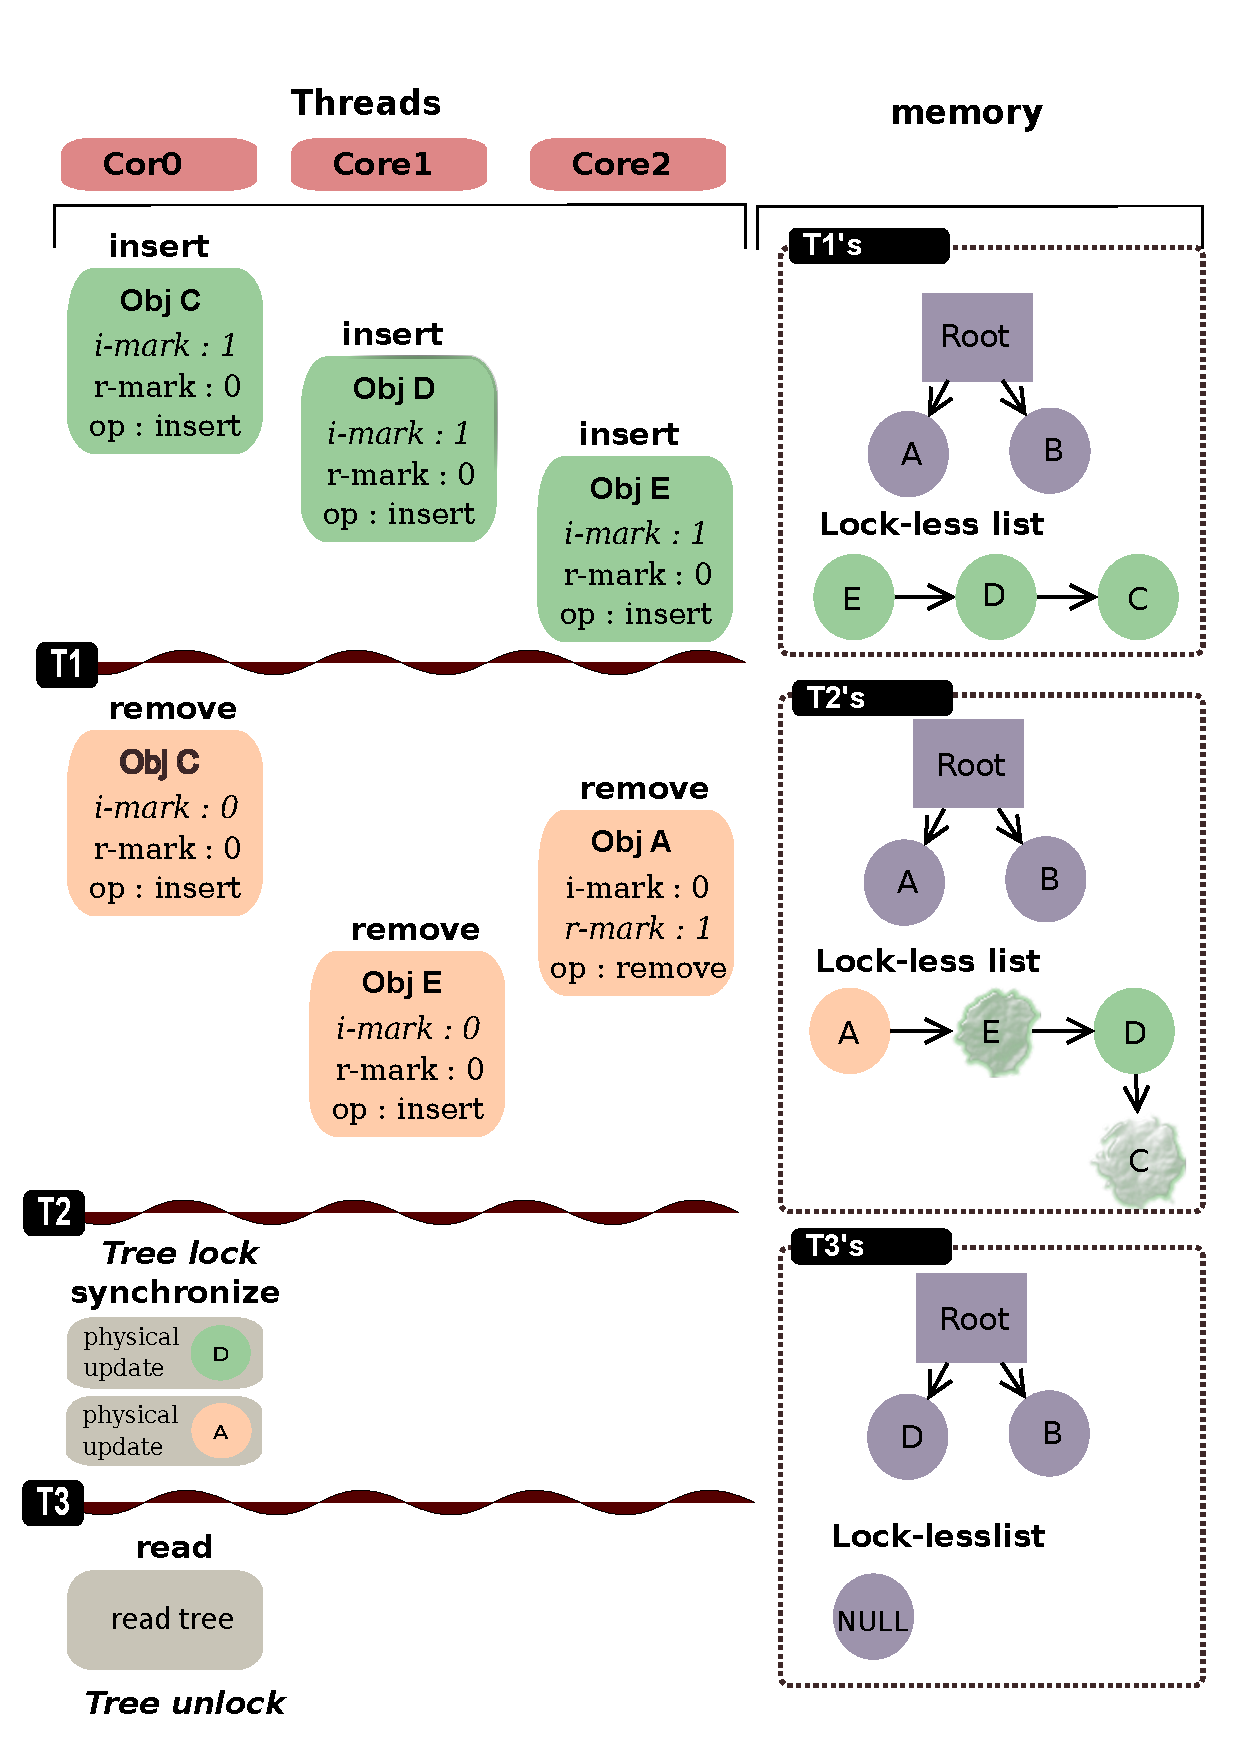
\includegraphics[width=0.5\textwidth,height=0.5\textheight,keepaspectratio]{fig/basic}
%  \end{center}
%  \caption{\deferu example showing six update operations and one read
%  operation. The execution flows from top to bottom. Memory represents original
%  data structure and logging queue at T1, T2 and T3, respectively.}
%  \label{fig:basic}
%\end{figure}

%\subsection{Approach}

%\deferu's scheme for concurrent update is proposed to overcome limitations
%of Linux kernel where 
%both insert and remove operations must not be invoked concurrently for the same
% object, but reads can be concurrently invoked with update.
%\deferu borrows ideas from Oplog's deferred processing and Harris' marking
% scheme.
%The reason is that Linux kernel's object management scheme differs from
% research-oriented data structure such as the lock-free and wait-free data
% structures~\cite{Harris2001Lockfree}~\cite{Fomitchev2004Lockfree}~\cite{Timnat2012}.
%For example, consider the Harris linked list, an insert operation inserts an 
%integer key into the data structure, but Linux kernel inserts their object link.
%The Linux kernel's list operations do not depend on key value.
%Furthermore, Harris linked list node's constructor can be invoked
%upon the insert function's scope, but Linux kernel's node is created on outside scope.
%In this regard, if duplicated remove operation occur, the Linux kernel may
%fail because their link pointer had been freed from destructor.
%Therefore, if a operation is an insert operation, the after operation must occurs 
%remove operation with regard to same object;the remove must execute after the 
%insert, or insert must execute after the remove.
%It means that updates such as insert and remove must not concurrently occur at
%the same object, but reads can occur concurrently.
%\deferu scheme inspires by this operation sequence, and inherits ideas
%from Oplog's deferred processing and Harris's marking scheme.

%\deferu's scheme for concurrent update inspires by Linux kernel's operation
%sequence.
%For example, consider a linked list in Linux kernel, if a operation is an insert
%operation, the after operation must occurs remove operation because Linux
%kernel's object management scheme differs from research-oriented data structure
%such as the lock-free and wait-free data
%structures~\cite{Harris2001Lockfree}~\cite{Fomitchev2004Lockfree}.
%Linux kernel's list operations do not depend on key value, but their 
%list operations depend on their object.
%These structure are their node's constructor can be invoked upon the insert
%function's scope, but Linux kernel's node is created on outside scope.
%In this regard, if duplicated remove operation occur, the Linux kernel may
%fail because their link pointer had been freed from destructor.
%Therefore, the remove must execute after the insert, or insert must execute
%after the remove.
%It means that updates such as insert and remove cannot concurrently occur at
%the same object, but reads can occur concurrently.
%\deferu scheme inspires by this operation sequence, and inherits ideas
%from Oplog's deferred processing and Harris's marking scheme.

%One important algorithm in our proposed novel concurrent update scheme is
%update-side absorbing operation that cancels duplicated operations for
% optimizations.
%A new remove operation, for example, may cancel an existing insert operation
%with regard to same object, so reader can eventually reads consistent data.
%Even though the Oplog's absorbing operation is invoked by
%read, \deferu's absorbing operation is fully invoked by update, so read-side
%performance is enhanced.

%The basic principle of update-side absorbing is that update uses atomic 
%marking operation for the object's mark field, which allows previous operation
% to cancel.
%For instance, if a new remove operation occurs after insert operation of the
%same object, \deferu does not store this operation in the lock-less
%list; instead, it changes the insert mark field to zero using the CAS.
%This mark is checked later when reading operation occurs and the operation log 
%maintained in the lock-less list is applied to original data structure
% atomically.
%This action may give effective update;however, the inserted operation log has
% remained in the lock-less list, so \deferu's reader checks the mark field
% when they convert operation log to original data structure atomically.

%figure : basic principle 
%Figure \ref{fig:basic} gives an example of deferred update with six update
%operations and one read operation.
%In this figure, execution flows from top to bottom.
%The data structure for \emph{physical update} is a tree, and initial values in
%the tree are node \code{A} and \code{B}.
%In contrast, the data structure for \emph{logical update} is lock-less list.
%In the top figure, \code{Core0}, \code{Core1} and \code{Core2} perform the
%logical insert operation to nodes \code{C}, \code{D} and \code{E},
% respectively.
%The logical inserts set the insert mark, and they then insert their
%nodes into lock-less list.
%In this case, none of the lock is needed because \deferu uses the lock-less
%list;all threads can execute the update concurrently.
%At \code{T1}, the tree contains node \code{A}
%and \code{B} and 
%the lock-less list contains node \code{E}, \code{D} and \code{C}.
%When removing the node \code{C}, the node \code{C}, whose mark field was marked
%by insert, atomically cleans up the insert marked field.
%At \code{T2}, the lock-less list contains nodes
%\code{A}, \code{E}, \code{D}, and \code{C}, and the marking field is zero for 
%nodes \code{E} and \code{C}.
%Before running the \code{synchronize} function, they need to lock the original
% tree's lock using the exclusive lock in order to protect the tree's
% operation.
%The \code{synchronize} migrates from lock-less list node to tree node, each of 
%which is the marked node, so nodes \code{A} and \code{D} are migrated.
%Finally, the tree contains nodes \code{D} and \code{B}, so the reader can read
% eventually consistent data.

%First, removing the cancelable operation at update point, \deferu uses the
% update side absorbing instead of read before absorbing.
%Therefore, read before operations in \deferu are fast because read-side
%absorbing operation is eliminated. 
%One notable difference between Oplog and \deferu is that 
%\deferu uses a light weight global queue with non-blocking synchronization 
%for update logs and eliminates time stamps while Oplog is dependent on 
%per-core logs with time stamps.
%By eliminating the global time stamps(hardware-dependent feature), \deferu is
% not dependent on hardware feature.
%Furthermore, update operations in \deferu are also fast because they use
%efficient update-side absorbing that eliminates traversal finding the
%cancelable operation.
%Furthermore, to optimize the log management and minimize the traversal
% overheads during reading, \deferu applies efficient update-side absorbing
% algorithm instead of read-side absorbing algorithm.

%\subsection{logical update}
%\begin{figure}[tb]
%\begin{obeylines}
%\begin{obeyspaces}
%function \(logical\_insert(obj, root) \):
%~~~If CAS(obj.del\_node.mark, 1, 0) $\ne$ 1:  
%~~~    obj.add\_node.mark $\gets$ 1
%~~~    If test\_and\_set\_bit(OP\_INSERT, obj.exist) $\ne$ true:
%~~~        set\_bit(OP\_INSERT, obj.used):
%~~~        obj.add\_node.op $\gets$ OP\_INSERT
%~~~        obj.add\_node.key $\gets$ obj
%~~~        obj.add\_node.root $\gets$ root
%~~~        add\_lock\_less\_list(obj.add\_node)
%~~~
%~~~
%function \(logical\_remove(obj, root) \):
%~~~If CAS(obj.add\_node.mark, 1, 0) $\ne$ 1:  
%~~~    obj.del\_node.mark $\gets$ 1 
%~~~    If test\_and\_set\_bit(OP\_REMOVE, obj.exist) $\ne$ true:
%~~~        set\_bit(OP\_REMOVE, obj.used):
%~~~        obj.del\_node.op $\gets$ OP\_REMOVE
%~~~        obj.del\_node.key $\gets$ obj
%~~~        obj.del\_node.root $\gets$ root
%~~~        add\_lock\_less\_list(obj.del\_node)

%\end{obeyspaces}
%\end{obeylines}
%\rule{\columnwidth}{0.5pt}
%\vspace{-\baselineskip}
%\caption{\deferu logical update algorithm. \code{logical\_insert} represents
% non-blocking insert function.
%It may be called by original insert position without locks. The fastpath is
% that when their object was removed by \code{logical\_remove},
% \code{logical\_insert} just changes node's marking field.}
%\label{fig:logicalupdate}
%\end{figure}

%The pseudo code for \deferu's \emph{logical update} is given in
%figure~\ref{fig:logicalupdate}.
%The \code{logical\_insert}, the concurrent update function, checks whether this
%object already has been removed by \code{logical\_remove}.
%If this object has been removed, \code{logical\_insert} initializes the marking
% field and then they return, which is fastpath.
%The marking field needs synchronization because this field in the
%\emph{logical update} is shared with the \emph{physical update}, so the CAS
% operation is needed.
%When the marking field has been initialized, they set the
%marking field, then they check whether or not this node already has been
% inserted in lock-less list.
%If the node does not exist in lock-less list, then they insert the node into
%lock-less list.

%\subsection{Physical update}
%\begin{figure}[tb]
%\begin{obeylines}
%\begin{obeyspaces}
%function \(synchronize\_ldu(obj, head) \):
%~~~If (head.first = NULL): 
%~~~    return; 
%~~~entry $\gets$ xchg(head.first, NULL);
%~~~for each list node:
%~~~    obj $\gets$ node.key
%~~~    clear\_bit(node.op, obj.exist)
%~~~    If CAS(node.mark, 1, 0) = 1:
%~~~         physical\_update(node.op, obj, node.root)
%~~~    clear\_bit(node.op, obj.used)
%~~~
%function \(physical\_update(op, obj, root) \):
%~~~If op = OP\_INSERT :  
%~~~    call real insert function(obj, root) 
%~~~Else If op = OP\_REMOVE :  
%~~~    call real remove function(obj, root) 

%\end{obeyspaces}
%\end{obeylines}
%\rule{\columnwidth}{0.5pt}
%\vspace{-\baselineskip}
%\caption{\deferu physical update algorithm. \code{synchronize\_ldu} may be
% called by reader and converts update log to original data structure
% traversing the lock-less list.}
%\label{fig:physicalupdate}
%\end{figure}

%The pseudo code for \deferu's \emph{physical update} is given in
%Figure~\ref{fig:physicalupdate}.
%First, they check whether lock-less list is an empty list or not, then they
%iterate the lock-less list.
%If the marking field has been set, they execute migration from
%lock-less to original data structure.
%Because the marking field in \emph{physical update} is shared with
% \emph{logical update}, the CAS operation is needed.
%They initialize the used field, which needs to protect the object from freed
% through destructor.
%The programmer must acquire locks on the \code{synchronize\_ldu} function,
%which migrates log to original data structure.
%Finally, the \code{physical\_update} executes original functions by using the
%operation log.
